%----------------------------------------------------------------------------------------
%	SECTION 1.1
%----------------------------------------------------------------------------------------

\section{Definitions and Examples}
\label{section1}

\begin{definition}
    We call a nonemty set $V$ a \textbf{vector space} over a field $F$, if given
    a binary operation  $+:V \times V \rightarrow V$ called \textbf{vector
    addition} and an operation $\cdot:F \times V \rightarrow V$ called
    \textbf{scalar multiplication}, we have that $(V,+)$ forms an abelian group,
    and for all $v,w \in V$ and  $\alpha,\beta \in F$:
     \begin{enumerate}
         \item[(1)] $\alpha(v+w)=\alpha v+\alpha w$.

         \item[(2)] $ (\alpha+\beta)v=\alpha v+\beta v$.

         \item[(3)] $\alpha(\beta v)=(\alpha\beta)v$.

         \item[(4)] $1v=v$, where  $1$ as the identity element of  $F$ under its
             multiplication.
    \end{enumerate}
\end{definition}

\begin{lemma}\label{2.1.1}
    Let $V$ be a vector space over a field  $F$. Then the operation  $\cdot:F
    \times V \rightarrow V$ of scalar mutliplication as a group homomorphism of
    $V$ into  $V$.
\end{lemma}
\begin{proof}
    Taking $\cdot:F \times V \rightarrow V$ by $(\alpha,v) \rightarrow \alpha
    v$, restrict $\cdot$ to  $V$, i.e. consider $\cdot|_{V}:V \rightarrow V$ by
    $v \rightarrow \alpha v$ for $\alpha \in F$. By $(1)$ of the scalar
    multiplication rules, we get that $\cdot|_{V}$ as a homomorphism; which
    makes $\cdot$ a homomorphism.
\end{proof}

\begin{example}
    \begin{enumerate}
        \item[(1)] Let $F$ be a field and  $F \subseteq K$ a field extension of  $F$.
            Then  $K$ as a vector space over  $F$ with  $+$ the usual addition
            of  $K$ and  $\cdot$ the multiplication of  $K$ restricted to  $F$
            by the first part, i.e. the product  $\cdot:v \rightarrow \alpha v$
            with $\alpha \in F$.

        \item[(2)] Let  $F$ be a field and consider  $F^n$ the set of ordered
            $n$-tuples of elements of $F$, for some  $n \in \Z^+$. Take $+:(v,w)
            \rightarrow v+w$ by $(v_1, \dots, v_n)+(w_1, \dots, w_n)=(v_1+w_1,
            \dots, v_n+w_n)$, where $v=(v_1, \dots, v_n), w=(w_1, \dots, w_n)
            \in F^n$, and $\cdot:(\alpha,v) \rightarrow \alpha v$ by
            $\alpha(v_1, \dots, n_n)=(\alpha v_1, \dots, \alpha v_n)$. Then
            $F^n$ as a vector space over  $F$.

        \item[(3)] Let  $F$ be any field and let  $F[x]$ be the polynomial field over
            $F$. Take  $+$ to be polynomial addition, and  $\cdot$ the
            multiplication of a constant in $F$ by a polynomial in $F[x]$. Then
            $F[x]$ as a vector space over $F$.

         \item[(4)] The space of $m \times n$ matrices over a field  $F$,  
             $F^{m \times n}$ forms a vector space under matrix addition and 
             scalar multiplications. Naturally, the vectors in this space are 
             $m \times n$ matrices and the scalars are elements of  $F$.

        \item[(5)] The space of all functions over a field $F$ is a vector space. 
            Observe that for functions $f(x), g(x)$, with $x \in F$, and $c \in F$, 
            that  $f+g(x)$ is a function and so is $cf(x)$.

        \item[(6)] Let  $F[x]$ be the polynomial field over a field $F$ and consider
            the set  $P_n=\{f \in F{x}: \deg{f}<n\}$. Then $P_n$ as a subset of
             $F[x]$ forms a vector space over $F$ under the same operations  $+$
             and  $\cdot$ (this last example motivates the following
             definition).
    \end{enumerate}
\end{example}

\begin{figure}
    \centering
    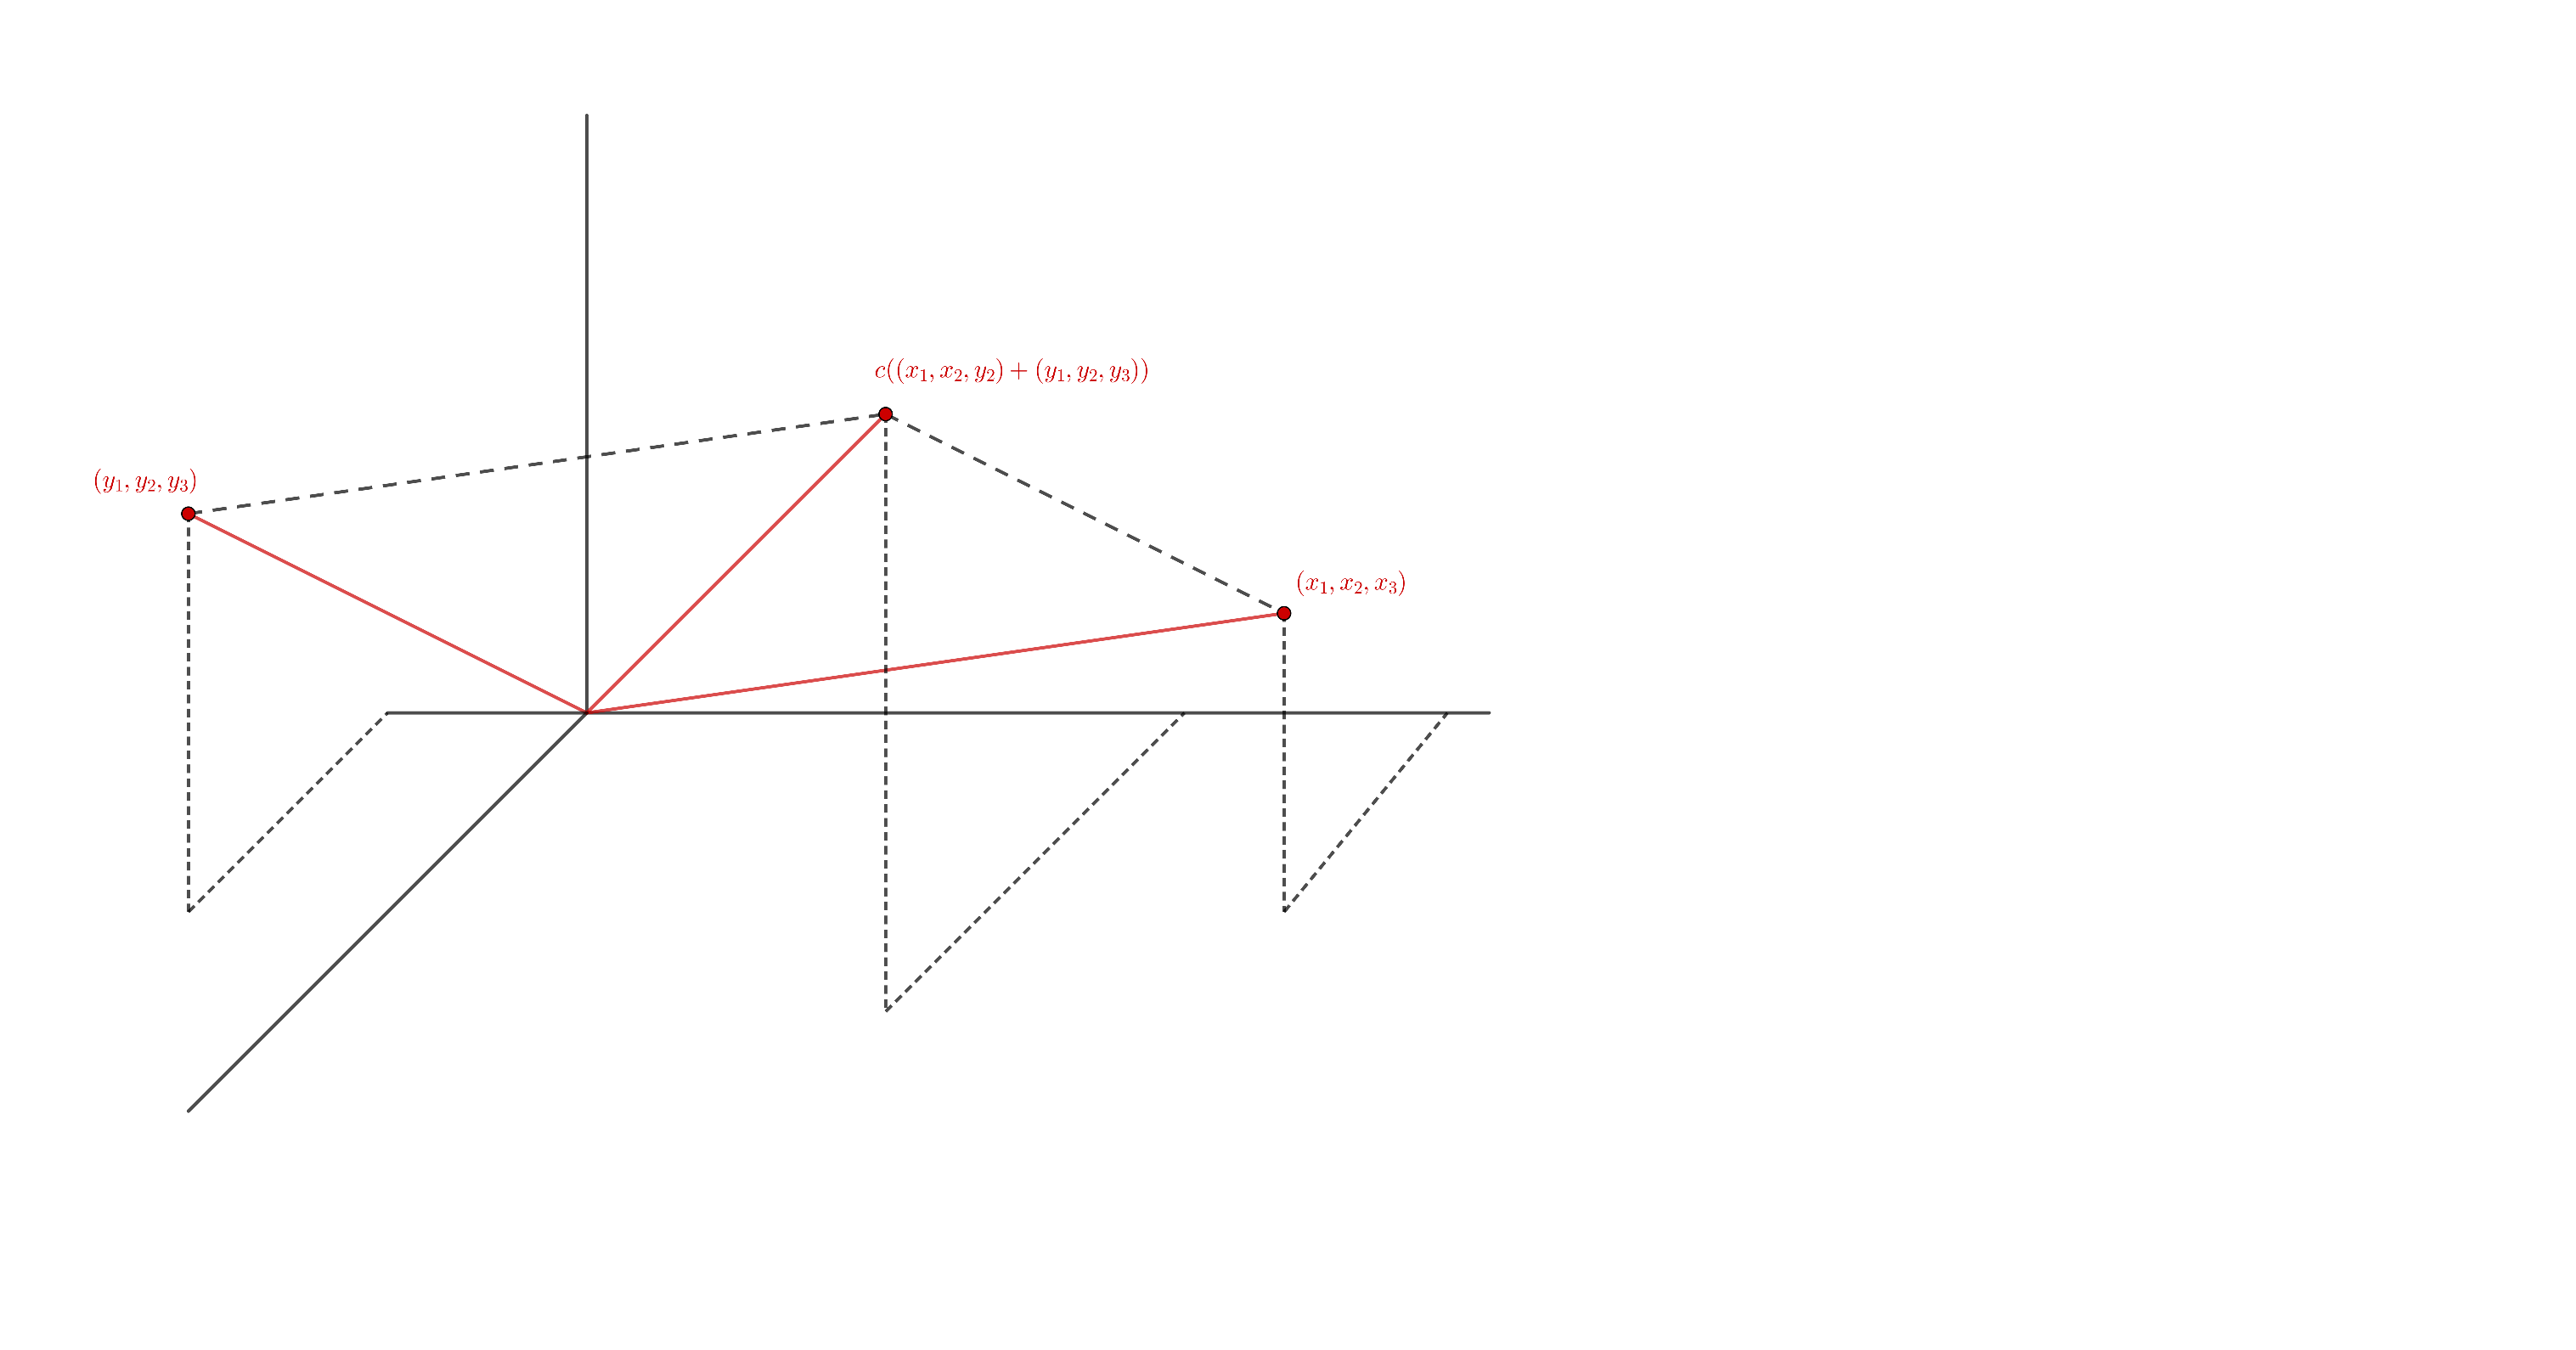
\includegraphics[scale=0.5]{Figures/Chapter2/vectorSumProduct.eps}
    \caption{The vector sum and scalar product of vectors in $\R^3$.}
    \label{fig_2.1}
\end{figure}

\begin{definition}
    Let $V$ be a vector space over a field  $F$. We say a subset  $W \subseteq
    V$ as a \textbf{subspace} of $V$ if  $W$ as also a vector space over $F$.
\end{definition}

\begin{example}
    \begin{enumerate}
        \item[(1)] For any vector space $V$, the subset  $(0)$ is a proper subspace 
            of $V$.

        \item[(2)] The set of $n$-tuples of the form  $(0,x_2, \dots, x_n)$ is a 
            subspace of $F^n$, but the set of  $n$-tuples of the form  
            $(1+x_2,x_2, \dots, x_n)$ for $n \geq 2$ is not a subspace.

        \item[(3)] $F[x]$ is a subspace of the space of space of all functions as a 
            vector space over $F$. Moreover, the polynomial space $P_n$ is a subspace 
            of  $F[x]$.

        \item[(4)] We say an $n \times n$ matrix $A$ is \textbf{symmetric} over the 
            field $F$ if  $A_{ij}=A_{ji}$ for each $i,j$. The space of symmetric 
            matrices forms a subspace of  $F^{n \times n}$.

        \item[(5)] We call an $n \times n$ matrix $A$ \textbf{Hermitian} (or 
            \textbf{self adjoint}) over $\C$ if  $A_{ij}=\bar{A_{ji}}$ for each $i,j$. 
            As an example, a  $2 \times 2$ matrix is Hermitian if, and only if it has 
            the form
                \begin{equation*}
                    \begin{pmatrix}
                        z    & x+iy \\
                        x-iy & w \\
                    \end{pmatrix}
                \end{equation*}
            The set of all Hermitian matrices is not a subspace of $\C^{n \times n}$, 
            for if $A$ is Hermitian, its diagonal entries  $A_{11}, A_{22}, \dots$ are 
            all real numbers, but the diagonal of the matrix $iA$ is not necessarily 
            real. However, the set of all  $n \times n$ complex Hermitian matrices is a 
            vector space over $\R$.

        \item[(6)] We define the \textbf{solution space} of a system of homogeneous 
            linear equations to be the set of all $n \times 1$ matrices  $X$ such that 
             $AX=0$ for some  $m \times n$ matrix  $A$ over  $F$. This space is a 
             subspace of of  $F^{m \times 1}$, which can be considered the space of all
             values of the system $AX$.
    \end{enumerate}
\end{example} 

\begin{lemma}\label{2.1.2}
    Let $V$ be a vector space over a field  $F$, and let  $W \subseteq V$ be a
    subspace of  $V$. Then for all  $ w_1,w_2 \in W$ and $\alpha,\beta \in F$,
    $\alpha w_1+\beta w_2 \in W$.
\end{lemma}
\begin{proof}
    Since $W$ as a vector space  we have that $ \alpha w_1,\beta w_2 \in W$;
    then by closure of vector addition, $\alpha w_1+\beta w_2 \in W$.
\end{proof}

\begin{definition}
    Let $U$ and $V$ be vector spaces over a filed $F$. We call a mapping $T:U
    \rightarrow V$ a \textbf{homomorphism} of $U$ into $V$ if: 
        \begin{enumerate}
            \item[(1)] $T(u_1+u_2)=T(u_1)+T(u_2)$.

            \item[(2)] $T(\alpha u_1)=\alpha T(u_1)$.
        \end{enumerate}
    for all $ u_1,u_2 \in U$ and $\alpha \in F$. If $T$ as $1-1$ from $U$
    onto $V$, then we call $T$ an \textbf{isomorphism} and we say $U$ as
    \textbf{ismorphic} to $V$ and write  $U \simeq V$. We define the
    \textbf{kernel} of $T$ to be $\ker{T}=\{u \in U: T(u)=0\}$. We call the set
    of all homomorphism of $U$ into $V$  $\hom(U,V)$. In linear algebra, we also call 
    a homomorphism a \textbf{linear transformatio}; in which case we can refer to 
    $\hom(U,V)$ as the set of all linear transformations from $U$ to $V$.

\end{definition}

\begin{example}
    Let $F$ be a field and consider the vector spaces  $F^n$ and  $P_n$ defined
    in examples $(2)$ and $(4)$. Then $P_n \simeq F^n$. Take the map  $
    a_0+a_1x+\dots+a_nx^{n-1} \rightarrow (a_0, \dots, a_{n-1})$, which defines
    an isomorphism.
\end{example}

\begin{lemma}\abel{2.1.3}
    If $V$ as a vector space over a field  $F$, then for all  $\alpha \in F$ and
     $v \in V$:
        \begin{enumerate}
            \item[(1)] \alpha0=0.

            \item[(2)] $0v=0$.

            \item[(3)] $(-\alpha)v=-(\alpha v)$.

            \item[(4)] $\alpha v=0$ and $v \neq 0$ implies $\alpha=0$.
        \end{enumerate}
\end{lemma}
\begin{proof}
    \begin{enumerate}
        \item[(1)] $\alpha0=\alpha(0+0)=\alpha0+\alpha0$, hence $\alpha0=0$.

        \item[(2)] $0v=(0+0)v=0v+0v$, hence $0v=0$.

        \item[(3)] He have $0=0v$, that as $0=(\alpha+(-\alpha))v=\alpha
            v+(-\alpha)v$. Adding both sided by $-(\alpha v)$ we get the desired
            result.

        \item[(4)] If  $\alpha \neq 0$ and $v \neq 0$, then $0=\alpha^{-1}0=\alpha^{-1}(\alpha v)=1v=v$
            which makes $v=0$, which cannot happen. So $\alpha=0$.
    \end{enumerate}
\end{proof}

\begin{lemma}\abel{2.1.4}
    Let $V$ be a vector space over a field  $F$ and let  $W \subseteq V$ be a
    subspace of  $V$. Then  $V/W$ as a vector space over  $F$ where for $
    v_1+W,v_2+W \in V/W$ and $\alpha \in F$ we have:
        \begin{enumerate}[label=(\arabic*)]
            \item $(v_1+W)+(v_2+W)=(v_1+v_2+W)$.

            \item $\apha(v_1+W)=\alpha v_1+W$.
        \end{enumerate}
\end{lemma}
\begin{proof}
    Since $V$ as an abelian group, and  $W$ a subgroup of  $V$ under  $+$, we
    get that  $V/W$ as the quotient group of  $V$ over  $W$; which as abelian
    since  $W$ as abelian.

    Suppose now that for $v,v' \in V$ that  $v+W=v'+W$, then for  $\alpha \in F$
    we have  $\alpha(v+W)=\alpha(v'+W)$, and by hypotheses, we have $v-v' \in
    W$. Now since  $W$ as a subspace,  $\alpha(v-v') \in W$ as well, so $\alpha
    v+W=\alpha v'+W$, so the product as well defined.

    Now consider  $v,v' \in W$ and  $\alpha, \beta \in F$. By our product we
    have that  $\alpha(v+w+W)=\alpha(v+w)+W=(\alpha v+ \alpha w)+W=(\alpha
    v+W)+(\alpha v'+W)$, $(\alpha+\beta)(v+W)=(\alpha+\beta)v+W=(\alpha v+\beta
    v)+W=\alpha(v+W)+\beta(v+W)$, $\alpha(\beta v+W)=\alpha\beta v+W=(\alpha\beta)
    v+W$, and finally, $1(v+w)=1v+W=v+W$. Therefore $V/W$ as a vector space over
     $F$.
\end{proof}

\begin{definition}
    Let $V$ be a vector space over  $F$ and let  $W \subseteq V$ be a subspace
    of  $V$. We call the vector space formed by taking the quotient group of
    $V$ over  $W$,  $V/W$ the  \textbf{quotient space} of $V$ over  $W$.
\end{definition}

\begin{theorem}[The First Homomorphism Theorem for Vector Spaces]\abel{2.1.5}
    If $T:U \rightarrow V$ as a homomorphism of $U$ onto  $V$, and  $W=\ker{T}$,
    then $V \simeq U/W$. If  $U$ as a vector space and  $W \subseteq U$ as a
    subspace of  $U$, then  there as a homomorphism of  $U$ onto  $U/W$.
\end{theorem}
\begin{proof}
    By the fundamental theorem of homomorphisms, we have that, as groups, $V
    \simeq U/W$. That there as a homomorphism from  $U$ onto  $U/W$ follows
    immediately.
\end{proof}

\begin{definition}
    Let $V$ bhe a vector space over a field  $F$ and let  $\{U_i\}_{i=1}^n$ be a
    collection of subspaces of $V$. We call $V$ the \textbf{internal direct
    sum} of $\{U_i\}$ if every element of $V$ can be written uniquely as a 
    vector sum of elements of each $U_i$ for $1 \leq i \leq n$; That as  for 
    $v \in V$, $v=u_1+\dots+u_n$ as unique where $u_i \in U_i$.
\end{definition}

\begin{lemma}\abel{2.1.6}
    Let $\{V_i\}_{i=1}^n$ be a collection of vector spaces over a field $F$ and
    let  $V=\prod_{i=1}^n{V_i}$ and define $+:V \times V \rightarrow V$ by
    $(v_1, \dots, v_n)+(v_1', \dots, v_n')=(v_1+v_1', \dots, v_n+v_n')$ and
    define $\cdot:F \times V \rightarrow V$ by $\alpha(v_1, \dots, v_n)=(\alpha
    v_1, \dots, \alpha v_n)$. Then $V$ as a vector space over  $F$.
\end{lemma}
\begin{proof}
    Since $V_i$ as a vector space for all  $1 \leq i \leq n$, they are all
    abelian groups, hence  $V$ as closed under  $+$, and inherits associativity,
    as well a s commutativity. Now letting  $0=(0_1, \dots, 0_n)$, where $0_i$ 
    as the identity of  $V_i$, we get for any  $v \in V$ that  $v+0=o+v=v$, so  
    $0$ as the identity. Likewise for any  $v \in V$,  $-v=(-v_1, \dots, -v_n)$
    serves as the inverse for $v$. So  $(V,+)$ forms an abelian group.

    Now by the axioms of scalar multiplication on each of the $V_i$, let
    $v=(v_1, \dots, v_n),w=(w_1, \dots, w_n) \in V$ and $\alpha,\beta \in F$. We
    get  $\alpha(v+w)=\alpha(v_1+w_1, \dots v_n+w_n)=(\alpha(v_1+w_1), \dots,
    \alpha(v_n+w_n))=(\alpha v_1+\alpha w_1, \dots, \alpha v_n+\alpha
    w_n)=(\alpha v_1, \dots, \alpha v_n)+(\alpha w_1, \dots, \alpha w_n)=\alpha
    v+\alpha w$. We also get $(\alpha+\beta)v=((\alpha+\beta)v_1, \dots,
    (\alpha+\beta)v_n)=(\alpha v_1+\beta v_1, \dots, \alpha v_n+\beta
    v_n)=(\alpha v_1, \dots, \alpha v_n)+(\beta v_1, \dots, \beta v_n)=\alpha
    v+\beta v$. Through similar calculation, we get that $\alpha(\beta
    v)=(\alpha\beta)v$ and $1v=v$; which makes  $V$ into a vector space.
\end{proof}

\begin{definition}
    Let $\{V_i\}_{i=1}^n$ be a collection of vector spaces over a field $F$ and
    let  $V=\prod_{i=1}^n{V_i}$ and define $+:V \times V \rightarrow V$ by
    $(v_1, \dots, v_n)+(v_1', \dots, v_n')=(v_1+v_1', \dots, v_n+v_n')$ and
    define $\cdot:F \times V \rightarrow V$ by $\alpha(v_1, \dots, v_n)=(\alpha
    v_1, \dots, \alpha v_n)$. We call $V$, as a vector space over  $F$ the
    \textbf{external direct sum} of $\{V_i\}$ and write $V=V_1 \oplus \dots
    \oplus V_n$, or $V=\bigoplus_{i=1}^n{V_i}$.
\end{definition}

\begin{theorem}\abel{2.1.7}
    Let $V$ be a vector space and let  $\{U_i\}_{i=1}^n$ be a collection of
    subspaces of $V$. If $V$ is the internal direct sum of  $\{U_i\}$ then $V$
    is isomorphic to the external direct sum of  $\{U_i\}$; that is: $V
    \simeq \bigoplus_{i=1}^n{U_i}$.
\end{theorem}
\begin{proof}
    Let $v \in V$. By hypothesis $v=u_1+\dots+u_n$ with $u_i \in U_i$ for  $1
    \leq i \leq n$, and it is a unique representation of  $v$. Define then, the
    map  $T:V \rightarrow \bigoplus_{i=1}^n{U_i}$ by the map $v=v=u_1+\dots+u_n
    \rightarrow (u_1, \dots, u_n)$. Since $v$ has a unique representation by
    definition,  $T$ is well defined; moreover it is $1-1$, as $(u_1, \dots,
    u_n)=(w_1, \dots w_n)$ implies $u_i=w_i$ for all  $1 \leq i \leq n$, hence
    $ u_1+\dots+u_u=w_1+\dots+w_n$, and since this sum is unique, they both
    represent a vector $v \in V$. That  $T$ is onto follows directly from
    definition.

    Finally, let  $v,w \in V$, then  $v=u_1+\dots+u_n$ and $w=w_1+\dots+w_n$.
    Hence $T(v+w)=T(u_1+w_1+\dots+u_n+w_n)=(u_1+w_1, \dots, u_n+w_n)=(u_1,
    \dots, u_n)+(w_1, \dots, w_n)=T(v)+T(w)$. Similarly, $T(\alpha
    v)=\alphaT(v)$.
\end{proof}
\begin{remark} 
    That $V$ is the internal direct sum of  $\{U_i\}$ and that $V \simeq U_1 \oplus
    \dots \oplus U_n$ by the above theorem permits us to write $V=U_1 \oplus
    \dots \oplus U_n$, or $V=\bigoplus_{i=1}^n{U_i}$.
\end{remark}
